\documentclass[Afour,sageh,times]{sagej}
\usepackage{moreverb,url}
\usepackage[colorlinks,bookmarksopen,bookmarksnumbered,citecolor=red,urlcolor=red]{hyperref}
\usepackage{graphicx}
\usepackage{caption}
\usepackage{subcaption}
\usepackage{multirow}
\usepackage{pdflscape}

\newcommand\BibTeX{{\rmfamily B\kern-.05em \textsc{i\kern-.025em b}\kern-.08em
T\kern-.1667em\lower.7ex\hbox{E}\kern-.125emX}}

\def\volumeyear{2025}

\begin{document}

\runninghead{Brodovsky MEMS-Nav}

\title{MEMS-Nav: A MEMS-Grade Dataset for Navigation Research}
\author{James Brodovsky\affilnum{1}, Philip Dames \affilnum{1}}
\affiliation{\affilnum{1}Temple University}
\corrauth{James Brodovsky, Temple University, Philadelphia, PA 19122, USA}
\email{jbrodovsky@temple.edu}

\begin{abstract}
This paper describes a dataset and toolbox for research and education in the field of navigation using MEMS-grade sensors. Many other such datasets either are collected in a fairly small scale laboratory or field setting (typical of the robotics and unmanned systems community), or they focus on high-end sensors (typical of the marine and aerospace communities). In contrast, this dataset splits the difference: it is collected on what might be the most ubiquitous type of sensor configuration --- the MEMS-grade IMU and GPS antenna on most modern cell phones --- and contains longer term trajectories comparable to the marine and aerospace communities. It's primary contribution it to provide a dataset that is both accessible and representative of real-world navigation problems for education as well as simulation of conditions of GPS/GNSS degradation, spoofing, and intermittent availability to enable research into alternative navigation techniques.
\end{abstract}

\keywords{inertial navigation, MEMS-grade sensors, dataset, IMU, GPS, GNSS}
\maketitle
\section{Introduction}
Inertial navigation systems (INSs) are widely used in various applications, including the robotics, aerospace, maritime, and automotive industries. These systems rely on a combination of inertial measurement units (IMUs) and external state feedback. The general architecture of a modern INS is to use the angular rate and specific force measurements from the IMU to propagate the state estimate over time. IMUs (even high quality ones) are nonetheless noisy sensors and integrating noise values twice eventually leads to substantial accumulation of error in the position and orientation estimates. This error is corrected by some sort of external state feedback often provided by the global navigation satellite system (GNSS), external beacons or markers, or by mapping landmarks via computer vision, lidar, or other sensing modalities. 

These industries apply the same basic Bayesian filtering techniques (Kalman filters, particle filters, et cetera) to fuse the inertial measurements with the external state feedback. However the scale of the navigation problem in each modality has facilitated different approaches to data collection and processing. While Bayesian navigation techniques have its origin in aerospace and maritime applications, the robotics and unmanned systems community has recently been making strides in the development of various autonomous navigation and localization applications using the same basic filters. This in turn has influenced the types of data collected by researchers in these fields.

An additional factor is the long term reliance and overall quality of traditional GNSS-INS systems. Even relatively inexpensive commercial grade systems can achieve high levels of accuracy in optimal conditions. Accuracy on the order of a few meters (or even centimeters) is common and is often sufficient for a platform that has footprint of tens or hundreds of meters. However, these systems' reliance on the GNSS makes them subject to various forms of GNSS signal degradation, including spoofing, intermittent availability, and other environmental factors that can affect the accuracy of the state feedback measurements. This has led to an increased interest in alternative methods of providing positioning, navigation, and timing (PNT) estimates that do not rely solely on GNSS and are thus subject to a single point of failure.

\section{{Problem}}
\subsection{Overview of available datasets}
Researchers and practitioners require access to quality datasets that capture or simulate the complexities of real-world navigation scenarios. Many such datasets exist that capture some aspects of these challenges, however they frequently rely on higher-end sensors, are proprietary even if still open-access (\cite{waymo}), or are collected in a fairly small scale laboratory or field setting. Additionally, the prominence of robotics and autonomy research groups publishing datasets in this field has led to a focus on datasets that are collected with the intent on developing a new capability (visual inertial odometry, simultaneous localization and mapping, et cetera) by leveraging and incorporating additional information about the local environment via additional sensors. This has also influenced the scale of datasets collected and it is common to see datasets that are collected on a small scale (such as in a building or laboratory) or in a small area (such as a campus or urban setting). A brief survey of these datasets is shown in Table \ref{tab:dataset_summary}.

\begin{table*}
  \caption{Short summary of some publicly available navigation datasets. Most datasets focus on providing feedback via the structure of the surrounding environment and are typically recorded on a laboratory, campus, or urban setting.}
  \label{tab:dataset_summary}
  \centering
  \begin{tabular}{|l|c|c|c|}
    \hline
    \textbf{Dataset} & \textbf{Platform} & \textbf{Ground Truth} & \textbf{Scale} \\
    \hline
    MIT DARPA & Car & GPS+INS & Urban \\
    \cite{mit-darpa} & & & \\
    \hline
    Ford Campus  & Car & GPS+INS & Campus \\
    \cite{ford-campus} & & & \\
    \hline
    KITTI  & Car and Robot & GPS+INS & Urban \\
    \cite{kitti} & & & \\
    \hline
    Oxford RobotCar  & Car & GPS+INS & Urban \\
    \cite{oxford-robotcar} & & & \\
    \hline
    KAIST Urban & Car & SLAM & Urban \\
    \cite{kaist-urban} & &  & \\
    \hline
    GFINS & Car & GPS+INS & Campus \\
    \cite{yampolsky2024multiple} & & & \\
    \hline
    New College & Handheld & SLAM & Campus \\
    \cite{new-college} & & & \\
    \hline
    Newer College & Handheld & SLAM & Campus \\
    \cite{newer-college} & & & \\
    \hline
    UMA-VI & Handheld & SLAM & Campus \\
    \cite{uma-vi} & & & \\
    \hline
    UZH FPV & UAV & GPS+INS & Campus \\
    \cite{uzh-fpv} & & & \\
    \hline
    TUM VI & Handheld & SLAM & Campus \\
    \cite{tum-vi} & & & \\
    \hline
    Penn Fast Flight & UAV & GPS & Laboratory \\
    \cite{upenn-fast-flight} & & & \\
    \hline
    EuRoC & UAV & Laser Tracker & Campus \\
    \cite{burri2016euroc} & & & \\
    \hline
    NTU VIRAL & UAV & Laser Tracker & Campus \\
    \cite{nguyen2022ntu} & & & \\
    \hline
    ANSFL & Mixed & GPS+INS & Regional \\ % This is probably the most similar and close in terms of use case
    \cite{ansfl} & & & \\
    \hline
  \end{tabular}
\end{table*}

In contrast, many traditional navigation problems do not have such information available to them in their environment. The aerospace and marine communities frequently operate in open environments with little availability of notable landmarks. Outside of the explicit context of visual flight rules, which is considered a basic and limited aviation operation condition, the reliance on inertial navigation and radio based position feedback is increasingly pronounced. Aviation in particular has a long history of using radio navigation aids such as very high frequency omnidirectional range station (VOR), non-directional beacon (NDB), and distance measuring equipment (DME) navigation aids to provide position feedback to pilots through manual calculations. In modern practice, these systems are being phased out in favor of attitude heading and reference systems (AHRS) and INSs that rely on the GNSS to provide position and orientation information. However, these systems can be subject to various forms of degradation, including spoofing, intermittent availability, and other environmental factors that can affect the accuracy of the position estimates.

On the opposite end of the use-case spectrum, the maritime community also faces similar issues with the reliance on GNSS or radio navigation aides. Surface vessels face similar challenges to aircraft but sub-surface vessels face the additional challenge of not being able to use the GNSS at all. Sub-surface vessels, ranging from military submarines to scientific unmanned underwater vessels, rely on an onboard INSs and other sensors to provide position and orientation information. Like all INS systems, these systems require external feedback in order to bound error. In contrast to surface vessels and aircraft, common means of obtaining such a position fix are typically at odds with the operational constraints of these platforms. The canonical example is that of a military submarine that must remain undetected and therefore cannot surface to obtain a GNSS fix.

\subsection{Challenges in collecting representative data}
Despite the breadth of datasets available, collecting representative data in GNSS-denied or degraded environments remains an open challenge. True denial scenarios—such as underwater or intentionally jammed conditions—are often logistically difficult, costly, or unsafe to replicate at scale. Even partial degradations, such as intermittent satellite visibility in urban canyons or under dense foliage, are highly environment-dependent and can be inconsistent from one experiment to another. This makes it difficult for researchers to obtain reproducible datasets that isolate the effects of GNSS degradation on navigation performance, particularly when using low-cost MEMS-grade sensors. As a result, the majority of available datasets continue to reflect ideal or near-ideal GNSS availability, limiting their utility for evaluating robustness in contested or constrained environments.

To address this gap, a complementary approach is to begin with high-quality, reproducible datasets and then systematically degrade the GNSS measurements in a controlled manner. This allows researchers to emulate spoofing, jamming, or intermittent availability while maintaining a consistent ground-truth reference. The ability to inject controlled degradations makes it possible to compare algorithms fairly, evaluate sensitivity to different types of GNSS disruptions, and benchmark alternative navigation strategies such as geophysical aiding or vision-based localization. Importantly, this reproducibility provides an avenue for broader adoption in both research and education: students and practitioners can explore realistic denial conditions without requiring access to specialized facilities or equipment, while developers can rigorously test robustness under a spectrum of degraded navigation scenarios

% In the aerospace and marine communities, this reliance on GNSS and radio navigation and it's limitations and vulnerabilities is a critical concern and has spurred interest in alternative PNT methods. One such family of methods is a form of complimentary navigation that leverages geophysical data to provide position feedback. This is typically done by comparing the inertial measurements from the IMU with geophysical data such as magnetic anomaly (\cite{magnav, tyren1982magnetic, canciani2016absolute,canciani2017airborne}), gravity anomalies (\cite{gravnav,jircitano1991gravity,kamgar1999vehicle,wang2016particle}), or terrain measurements (\cite{}). By comparing the inertial measurements with the geophysical data, it is possible to estimate the position of the platform without relying on GNSS or radio navigation aids. This approach has been shown to be effective in a variety of applications, including aircraft, submarines, and unmanned underwater vehicles.

% Geophysical navigation methods do have a limitaion due to the resolution of the commonly used public maps (terrain: \cite5{SANDWELL20211059}, gravity anomaly: \cite{EGM2008}, magnetic anomaly: \cite{wdmam}). These maps are typically at a coarse resolution. The terrain map has the highest resolution of 15 arc-seconds (approximately 452 meters) where as gravity anomaly and magnetic anomaly are much lower resolution (1 arc minute and 3 arc minutes; approximately 1,852 and 5,556 meters respectively) and therefore require a larger area to be covered in order to provide sufficient information for accurate position estimation. As a result, geophysical navigation methods are typically only viable on longer duration longer distance trajectories.

\section{The MEMS-Nav Dataset and Strapdown Simulator}
This paper presents the MEMS-Nav dataset and an accompanying toolbox and simulator for strapdown inertial navigation systems and GNSS degradation simulation. The dataset, toolbox, and simulator are designed to be both accessible and representative of real-world conditions. The dataset is collected using MEMS-grade sensors, which are commonly found in modern smartphones and other consumer electronics. This makes the dataset more relatable and applicable to a wider audience, including researchers and developers working with low-cost navigation systems.

The dataset was collected using a variety of smartphones all of which had an internal IMU board that contain accelerometers, gyroscopes, magnetometers, and a barometer, paired with a GPS antenna using the Sensor Logger application (\cite{awesome-sensor-logger}). There were a variety of vehicles used to collect the data but the majority of the data was collected using a car and typically on highway driving conditions. The raw recording measurements were synchronized and contain the following measurements from GNSS processing:\begin{itemize}
  \item \textbf{Latitude} --- WGS 84 degrees latitude
  \item \textbf{Longitude} --- WGS 84 degrees longitude 
  \item \textbf{Altitude} --- WGS 84 altitude in meters
  \item \textbf{Speed} --- Ground speed in meters per second
  \item \textbf{Horizontal Accuracy} --- Horizontal accuracy in meters
  \item \textbf{Vertical Accuracy} --- Vertical accuracy in meters
\end{itemize} from IMU processing: \begin{itemize}
  \item \textbf{Bearing} --- Magnetic bearing (compass) in degrees
  \item \textbf{Bearing Accuracy} --- Bearing accuracy in degrees
  \item \textbf{Angular Rates} --- Angular rates in radians per second (\verb|gyro_x|, \verb|gyro_y|, \verb|gyro_z|)
  \item \textbf{Magnetic Field Vector} --- Magnetic field in microteslas (\verb|mag_x|, \verb|mag_y|, \verb|mag_z|)
  \item \textbf{Gravity Vector} --- Gravity vector in meters per second squared (\verb|grav_x|, \verb|grav_y|, \verb|grav_z|)
  \item \textbf{Pressure} --- Barometric pressure in millibars
\end{itemize} and derived quantities:\begin{itemize}
  \item \textbf{Relative Altitude} --- meters, relative change in altitude derived from barometric pressure
  \item \textbf{Attitude (Euler Angles)} --- roll, pitch, and yaw in degrees
  \item \textbf{Attitude (Quaternion)} --- quaternion representation of the attitude (\verb|qx|, \verb|qy|, \verb|qz|, \verb|qw|)
  \item \textbf{Linear Acceleration} --- Linear acceleration in meters per second squared (\verb|acc_x|, \verb|acc_y|, \verb|acc_z|)
\end{itemize}

The dataset has three primary contributions. First, the preprocessed input recordings that can be used for the development of alternative positioning, navigation, and timing (AltPNT) technology. Second, a `truth' dataset that is generated using a strapdown mechanization approach with GNSS position and velocity measurements as well as barometric altitude fused via an Unscented Kalman Filter INS. This truth dataset is intended to provide a reference `ground truth' for evaluating the performance of other navigation algorithms. The input dataset and corresponding truth dataset can be used as a benchmark for developing and testing new algorithms as well as an educational resource for autonomous navigation courses. Third, the dataset contains a variety of simulated environmental conditions related to the GNSS signal (e.g. an intermittent signal due to jamming, a degraded signal due to interference, et cetera) that serve as examples of what the simulator is capable of generating. This is intended to provide a useful resource for researchers investigating GNSS-denied navigation techniques.

\subsection{Reference INS Implementation}
When dealing with noisy sensors and probabilistic navigation and state estimation techniques a word must be said about what is considered `truth' and what you compare your estimates against to measure error. Fundamentally, these techniques all rely on quantities that are considered noisy and probabilistic as such it is important to establish both an estimate and a certainty. 

Frequently, a highly accurate external reference, such as motion capture systems or GNSS measurements is used and this is perfectly acceptable when the goal is to evaluate a navigation or simultaneous localization and mapping (SLAM) system that does not use these measurements. Additionally, Bayesian filtering techniques often produce more accurate and more confident estimates from combining multiple noisy measurements. Both the raw measurements (the `input' dataset) and the filtered dataset (`truth') are provided as a reference. User are free to use either the GNSS measurements or the estimated state as their source of truth for error comparison.

\subsubsection{Coordinate and state definitions}
The INS is implemented as a strapdown mechanization in the local level frame. The local level frame and strapdown mechanization are widely implemented and provide a common introductory framework for INS development. The local level frame is defined as a frame that is tangent to the Earth's surface with axes pointed towards the Earth's north pole, eastward direction, and a vertical axis pointing normal to the surface. These axes are typically configured as a right handed orthonormal frame of North-East-Down or East-North-Up. The typical nine-state NED/ENU navigation state vector is used in this implementation. The state vector is defined as:
\[
x = \left[p_n, p_e, p_d, v_n, v_e, v_d, \phi, \theta, \psi \right] 
\]
where: \begin{itemize}
  \item \(p_n\), \(p_e\), and \(p_d\) are the WGS84 geodetic positions (degrees latitude, degrees longitude, meters relative to the ellipsoid)
  \item \(v_n\), \(v_e\), and \(v_d\) are the local level frame (NED/ENU) velocities (m/s) along the north axis, east axis, and vertical axis 
  \item \(\phi\), \(\theta\), and \(\psi\) are the Euler angles (in radians) representing the orientation of the body frame relative to the local level frame (XYZ Euler rotation)
\end{itemize}

\subsubsection{Strapdown equations in the Local-Level Frame}
The reference INS implements the strapdown mechanization equations in the Local-Level Frame according to \cite{groves}. These equations form the basis of the forward propagation step (motion/system/state-transition model) of the INS's filter. The forward mechanization equations are executed in three steps: the attitude update, the velocity update, and the position update. 

First, given a direction-cosine matrix \(C_b^n\) representing the attitude of the platform's body frame (\(b\)) with respect to the local level frame (\(n\)), the transport rate \(\Omega_{en}^n\) representing the rotation of the local level frame with respect to the Earth-fixed frame (\(e\)), the Earth's rotation rate \(\Omega_{ie}^e\), and the angular rate \(\Omega_{ib}^b\) representing the rotation of the body frame with respect to the inertial frame (\(i\)), the attitude update equation is given by:
\[
C_b^n(+) \approx C_b^n(-) \left( I + \Omega_{ib}^b t \right) - \left( \Omega_{ie}^e - \Omega_{en}^n \right) C_b^n(-) t
\]
where \(t\) is the time differential and \(C(-)\) is the prior attitude. These attitude matrices are then used to transform the
specific forces from the IMU:
\[
f_{ib}^n \approx \frac{1}{2} \left( C_b^n(+) + C_b^n(-) \right) f_{ib}^b
\]
Next, the velocity is updated by:
\[
v(+) \approx v(-) + \left( f_{ib}^n + g_{b}^n - \left( \Omega_{en}^n - \Omega_{ie}^e \right) v(-) \right) t
\]
Finally, the base position states are updated in three steps. First update the altitude:
\[
p_d(+) = p_d(-) + \frac{1}{2} \left( v_d(-) + v_d(+) \right) t
\]
Next, update the latitude:
\[
p_n(+) = p_n(-) + \frac{1}{2} \left( \frac{v_n(-)}{R_n + p_d(-)} + \frac{v_n(+)}{R_n + p_d(+) } \right) t
\]

Finally, update the longitude:

\begin{equation*}
    \begin{split}
      p_e(+) = p_e(-) + \frac{1}{2} \dots \\ \left( \frac{v_e(-)}{(R_e + p_d(-)) \cos(p_n(-))} + \frac{v_e(+)}{(R_e + p_d(+)) \cos(p_n(+))} \right) t
    \end{split}
\end{equation*}

The filter then updates the mean and covariance using a loosely coupled architecture. In such an architecture, the GNSS reciever produces a position and velocity estimate that is directly compared to the filter's state estimate. Additionally the onboard barometer's estimate of relative altitude is included to provide additional feedback into the vertical channel.

\subsection{GNSS Degradation Models}

To enable systematic evaluation under contested navigation conditions, the toolbox provides models that act at two layers: scheduling (when GNSS fixes are delivered) and fault injection (how those fixes are corrupted). These can be used independently or in combination, allowing the same high-quality dataset to be replayed under a wide variety of degraded scenarios.  

At the scheduling level, three modes are supported. The \emph{pass-through} scheduler emits all measurements without modification and serves as a baseline for `ideal' conditions. A \emph{fixed-interval} scheduler outputs fixes at a prescribed interval (e.g., every 10~s), discarding intermediate updates to mimic reduced-rate operation caused by jamming, low-power duty cycling, or bandwidth constraints. The \emph{duty-cycle} scheduler alternates between ON and OFF windows, reproducing periodic outages similar to those encountered in tunnels or urban canyons. These mechanisms provide control over temporal availability and can be tuned to match operational conditions.  

At the measurement level, the toolbox implements several distinct corruption models. The \emph{degraded} model applies autoregressive (AR(1)) noise processes to position and velocity, combined with inflated covariance reports. This represents conditions such as multipath or low-SNR reception, where GNSS remains available but with reduced fidelity. The \emph{slow bias} model represents ``soft spoofing'': a gradual drift in position and velocity along a chosen direction, potentially with stochastic and rotational components. Such errors remain plausible to a Bayesian filter and are therefore particularly insidious. The \emph{hijack} model, in contrast, represents ``hard spoofing'': a constant offset applied abruptly during a specified time window, displacing the estimated trajectory onto a parallel but false path. Finally, a \emph{combination} model allows these effects to be chained together, such as combining a slow drift with a subsequent spoofing window, to emulate complex multi-stage attacks.

\begin{table*}
\centering
\caption{Summary of GNSS degradation models implemented in the toolbox.}
\begin{tabular}{|l|c|p{6cm}|c|}
\hline
\textbf{Layer} & \textbf{Model} & \textbf{Description} & \textbf{Representative Scenario} \\
\hline
\multirow{3}{*}{Scheduling} 
  & Pass-through   & Emit all fixes unchanged. & Baseline / truth replay \\
  & Fixed-interval & Emit fixes only at specified intervals; drop others. & Jamming, low-power mode \\
  & Duty-cycle     & Alternate ON/OFF windows of availability. & Tunnel, urban canyon \\
\hline
\multirow{5}{*}{Fault Model}
  & None           & No corruption of measurement content. & Baseline \\
  & Degraded       & AR(1) correlated noise in position \& velocity; inflated covariance. & Multipath, interference \\
  & Slow bias      & Gradual drift in N/E position \& velocity; optional random walk and rotation. & Soft spoofing \\
  & Hijack         & Constant offset applied during a time window. & Hard spoofing attack \\
  & Combo          & Sequential application of multiple models. & Multi-stage spoofing/jam \\
\hline
\end{tabular}
\end{table*}

\subsection{An example}

An example trajectory from the dataset is shown in Figure \ref{fig:example_trajectory}. This trajectory was collected using a car on predominantly highway driving conditions. The trajectory is approximately 90 minutes long and covers a distance of approximately 113 kilometers. 

\begin{figure*}
  \centering
  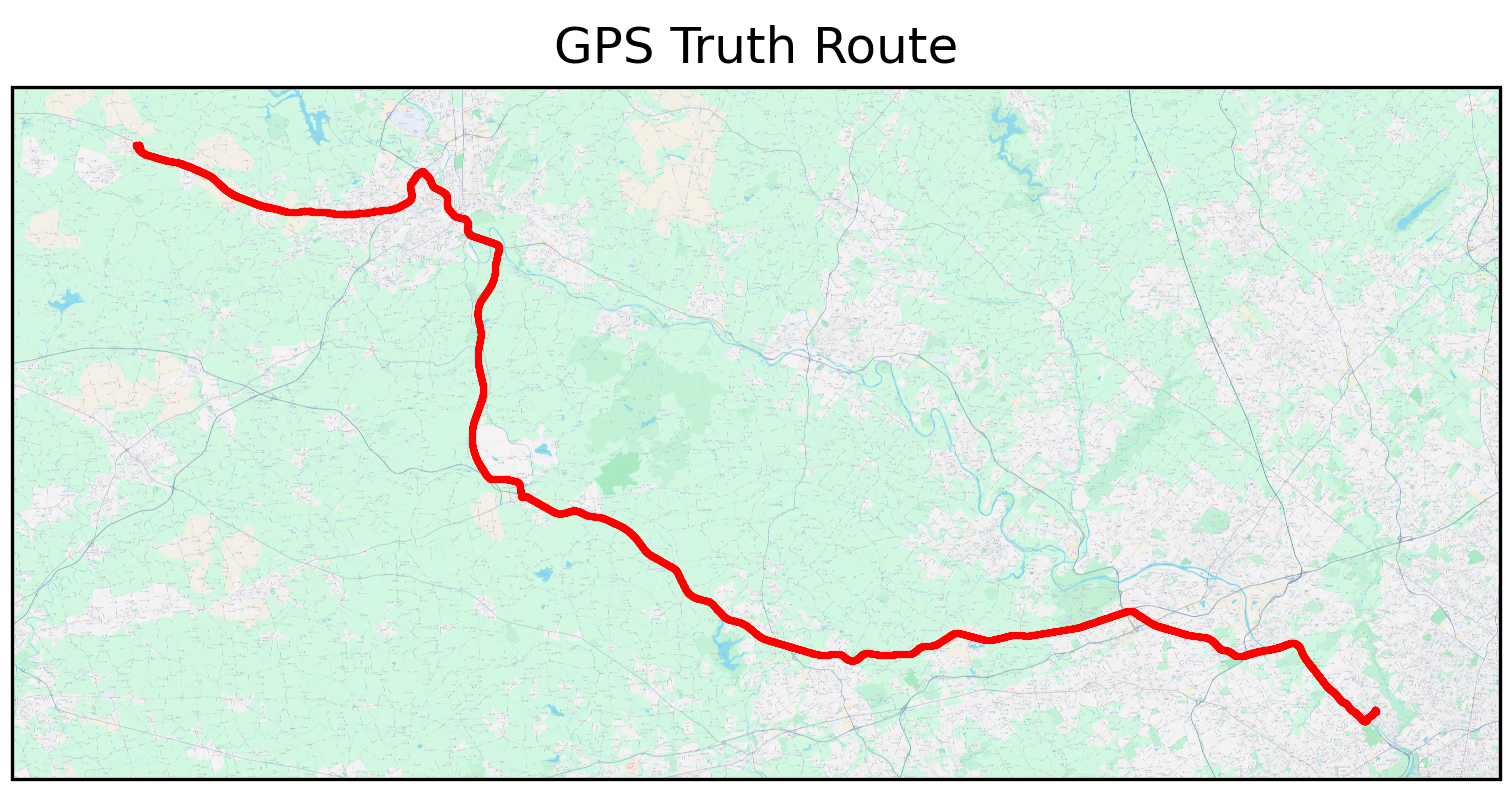
\includegraphics[width=\textwidth]{images/route_gps.png}  
  \caption{Example trajectory from the MEMS-Nav dataset.}
  \label{fig:example_trajectory}
\end{figure*}

Using the ``passthrough'' scheduler and no fault injection, the reference INS produces the position error shown in Figure \ref{fig:truth_error}. The position error is calculated as the difference between the GNSS position measurements and the INS position estimate using a haversine distance. 

\begin{figure*}
  \centering
  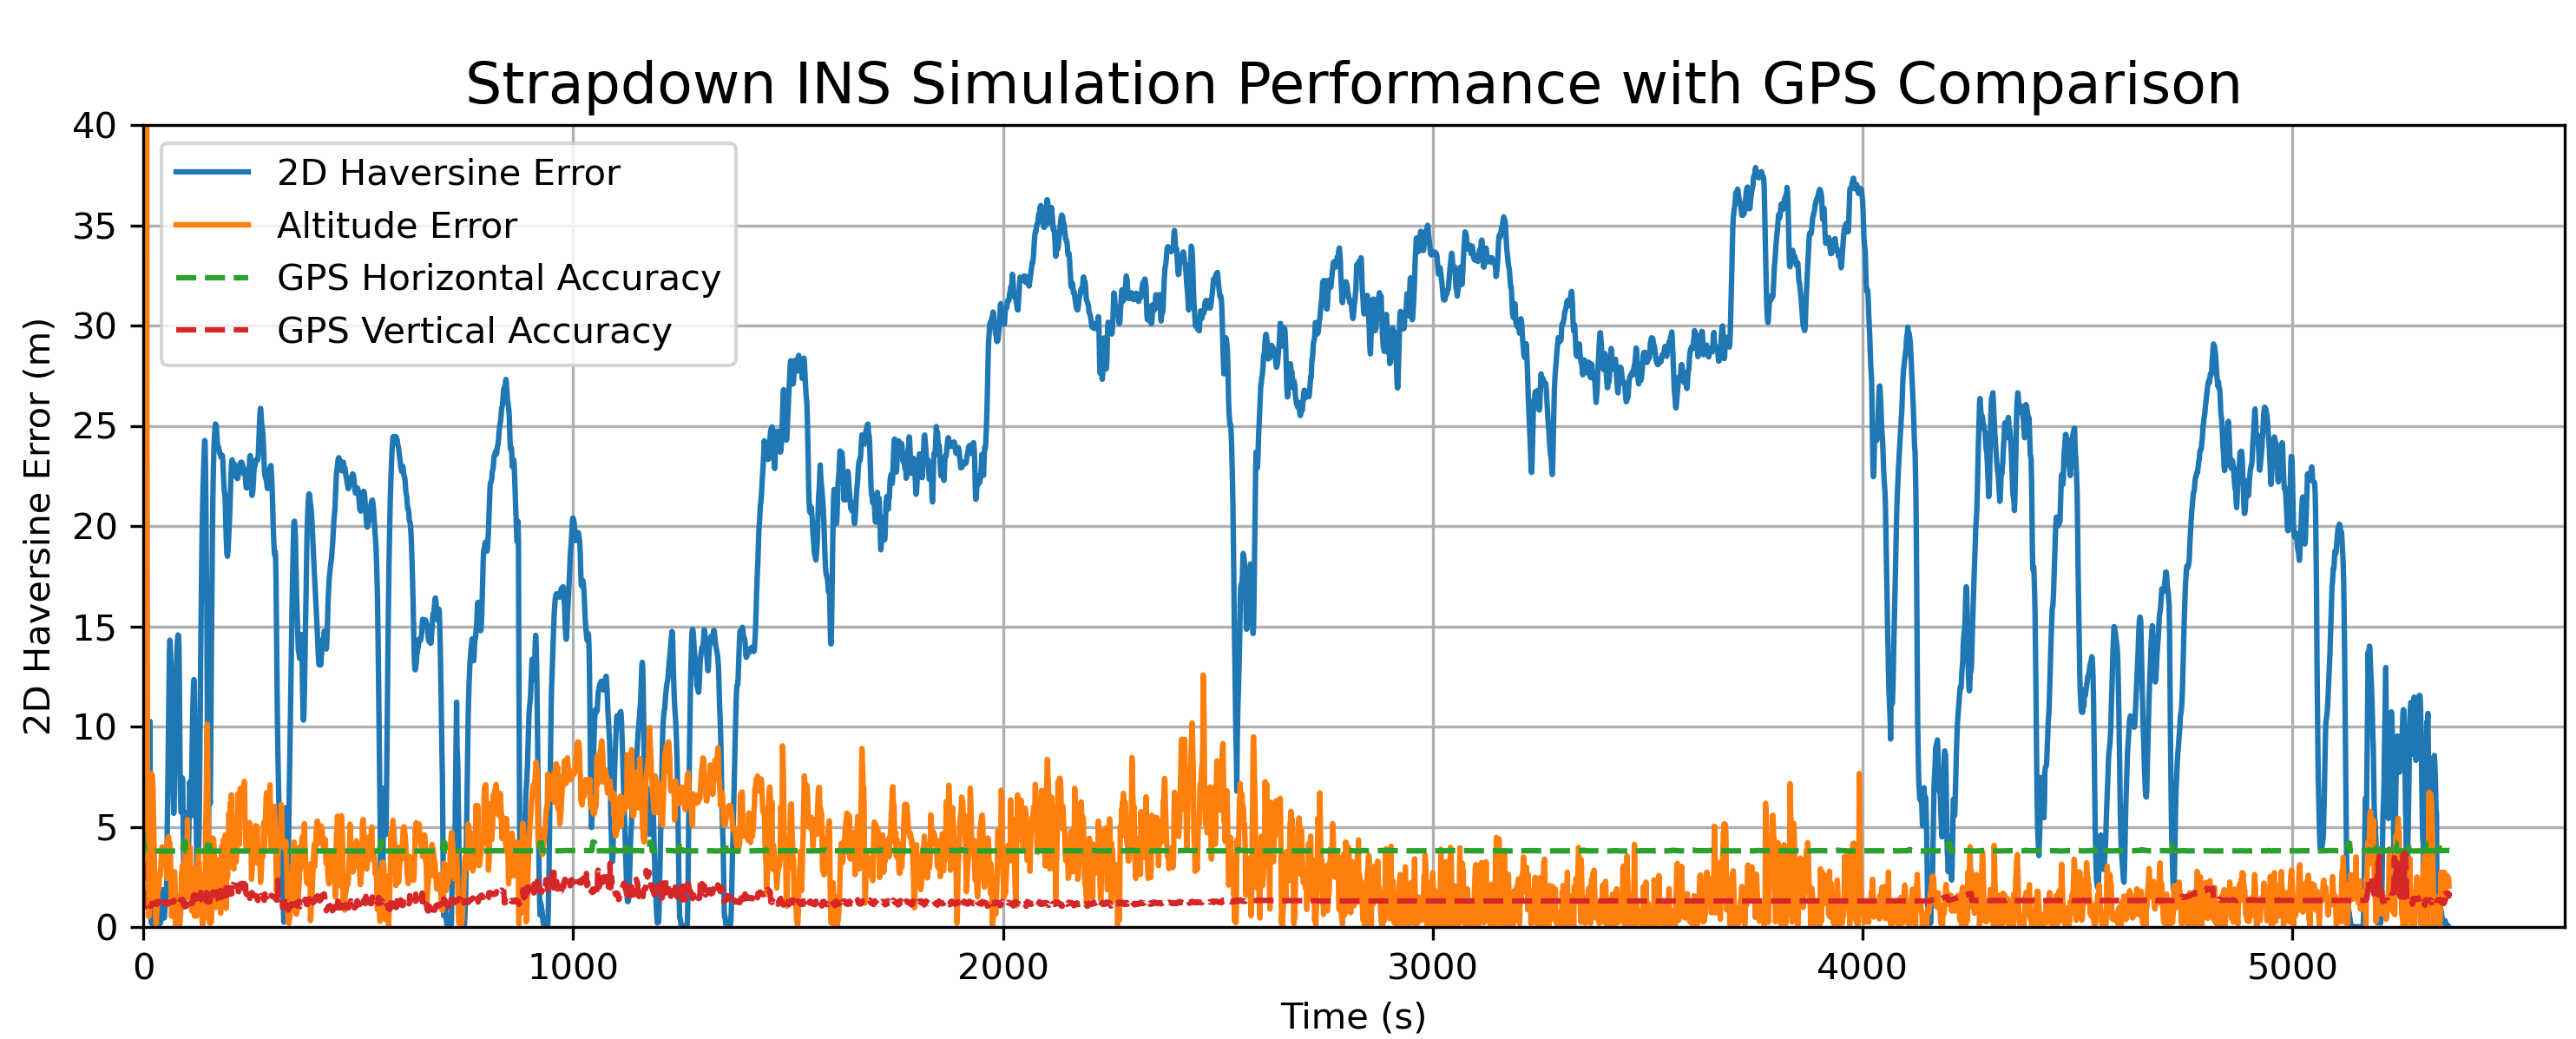
\includegraphics[width=\textwidth]{images/performance.png}  
  \caption{Position error of the reference ``truth'' trajectory that fuses IMU and GNSS measurements.}
  \label{fig:truth_error}
\end{figure*}

While not necessarily as precise as GPS or a high-end INS, the reference trajectory is nonetheless a substantial improvement over using the IMU alone, and is at times able to achieve a horizontal estimate that is more accurate than the GNSS measurements themselves. The barometric altitude measurements also provide a substantial improvement over the GNSS altitude measurements and IMU, as the vertical channel is often very noisy. This reference INS trajectory can therefore be used as a reasonable ground truth for evaluating the performance of other navigation algorithms.

\begin{figure*}
  \centering
  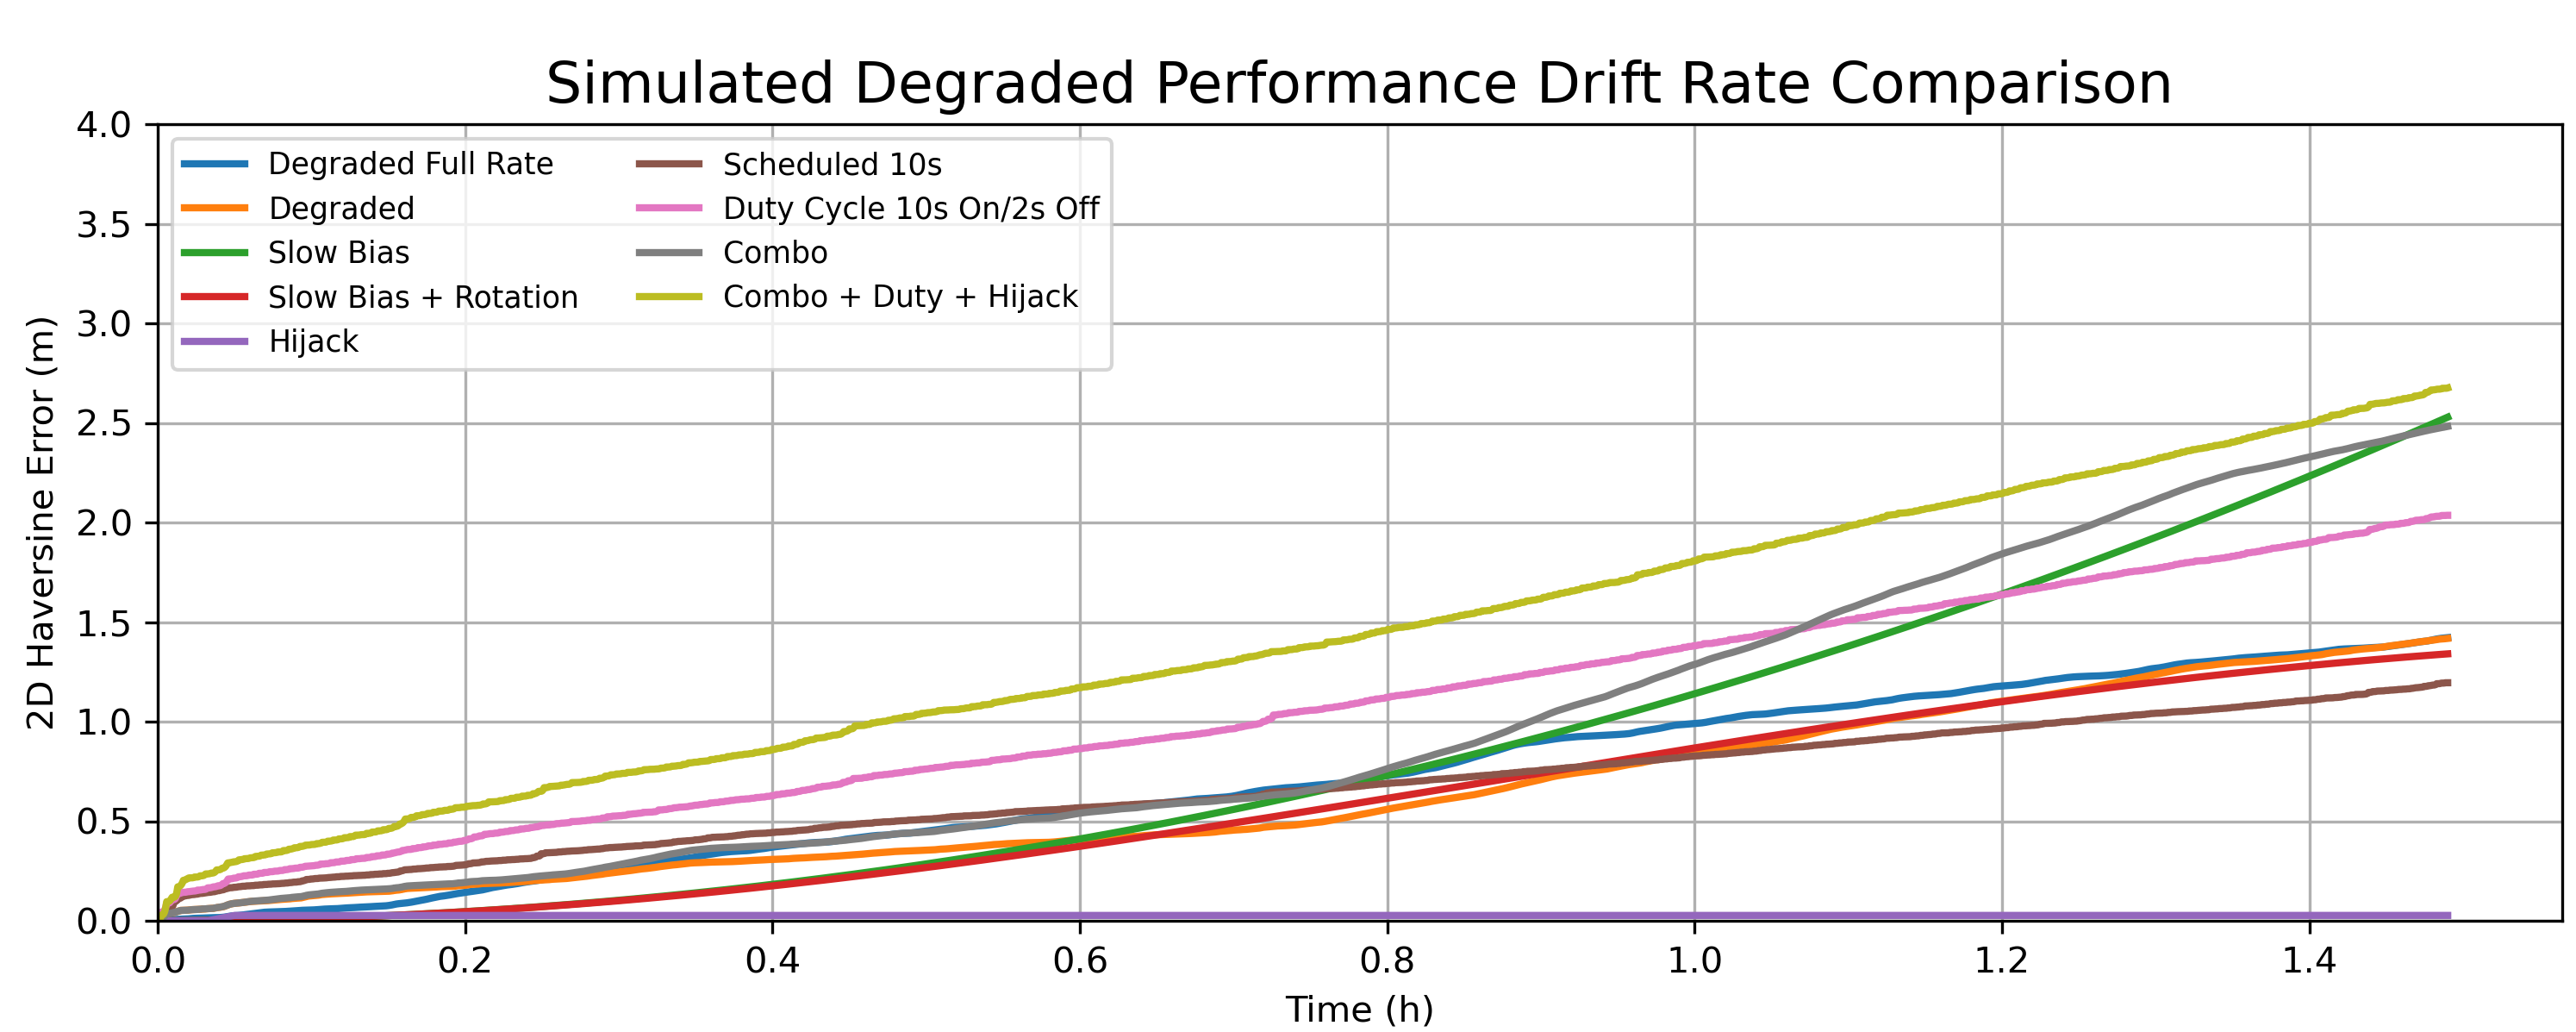
\includegraphics[width=\textwidth]{images/performance_comparison.png}  
  \caption{Position error under the ``degraded'' GNSS model.}
  \label{fig:degraded_performance}
\end{figure*}

Using the same input recording, we then subject the GNSS measurements to a variety of degradation models as shown in Table \ref{tab:degradation_models}. The resulting position errors are normalized to be with respect to distance traveled.

\begin{table}[]
\centering
\caption{Summary of GNSS degradation models applied to the example trajectory.}
\label{tab:degradation_models}
\begin{tabular}{|p{2cm}| p{5cm}|}
  \hline
  \textbf{Condition} & \textbf{Description} \\
  \hline
  Degraded & AR(1) correlated noise in position \& velocity; inflated covariance. \\
  \hline
  Degraded + intermittent GNSS & AR(1) correlated noise in position \& velocity; inflated covariance. GNSS fixes only every 5 seconds. \\
  \hline
  Slow bias & Gradual drift in N/E position \& velocity; random walk and rotation. \\
  \hline
  Slow bias with rotation & Gradual drift in N/E position \& velocity with rotation. \\
  \hline 
  Hijack & Constant offset applied during a time window (between 30 and 60 minutes). \\
  \hline
  Reduced rate & GNSS fixes only every 10 seconds. \\
  \hline
  Duty cycle & GNSS available for 10 seconds, then unavailable for 2 seconds. \\
  \hline
  Combination degraded and slow bias & AR(1) correlated noise in position \& velocity; inflated covariance. Gradual drift in N/E position \& velocity; fixes applied every 5 seconds. \\
  \hline
\end{tabular}
\end{table}


\section{Conclusion}

This paper presents the MEMS-Nav dataset, which is designed to be both accessible and representative of real-world conditions. The dataset is collected using MEMS-grade sensors, which are commonly found in modern smartphones and other consumer electronics. This makes the dataset more relatable and applicable to a wider audience, including researchers and developers working with low-cost navigation systems. The dataset is preprocessed and includes a `truth' dataset generated using a strapdown mechanization approach with GNSS position and velocity measurements as well as barometric altitude fused via an Unscented Kalman Filter INS. This truth dataset is intended to provide a reference `ground truth' for evaluating the performance of other navigation algorithms. The input dataset and corresponding truth dataset can be used as a benchmark for developing and testing new algorithms as well as an educational resource for autonomous navigation courses. 

Additionally, the dataset contains a variety of simulated environmental conditions related to the GNSS signal (e.g. an intermittent signal due to jamming, a degraded signal due to interference, et cetera) that serve as examples of what the simulator is capable of generating as well as pre-packaged scenario results for testing. This is intended to provide a useful resource for researchers investigating GNSS-denied navigation techniques.

The dataset, toolbox, and simulator are available at \url{https://github.com/jbrodovsky/strapdown-rs} with the input files available under the releases section of the repository. Alternatively, the processed files composing the dataset are available at \url{https://github.com/jbrodovsky/mems-nav-dataset}. The raw data files are available upon request to the corresponding author.

\begin{acks}
The author would like to thank the following people for their assistance in recording the raw data files: Beth Brodovsky, Jeremy Brodovsky, Monica Brodovsky, Bill Siegl, and Alkesh Kumar.
\end{acks}


\bibliographystyle{SageH}
\bibliography{references.bib}
\end{document}
